\documentclass[12pt,a4paper]{report}

% ══════════════════════════════════════════════════════════════
% PACKAGES
% ══════════════════════════════════════════════════════════════
\usepackage[utf8]{inputenc}
\usepackage[T1]{fontenc}
\usepackage[french]{babel}
\usepackage{geometry}
\usepackage{graphicx}
\usepackage{amsmath,amssymb}
\usepackage{booktabs}
\usepackage{tabularx}
\usepackage{multirow}
\usepackage{longtable}
\usepackage{float}
\usepackage{caption}
\usepackage{subcaption}
\usepackage{listings}
\usepackage{xcolor}
\usepackage{hyperref}
\usepackage{fancyhdr}
\usepackage{titlesec}
\usepackage{tocloft}
\usepackage{setspace}
\usepackage{parskip}
\usepackage{enumitem}
\usepackage{tikz}
\usetikzlibrary{shapes.geometric, arrows.meta, positioning, fit, calc}

\graphicspath{{diagrams/}}

\geometry{
  top=2.5cm,
  bottom=2.5cm,
  left=3cm,
  right=2.5cm
}

\onehalfspacing

% ── Hyperref setup ──
\hypersetup{
  colorlinks=true,
  linkcolor=blue!60!black,
  citecolor=green!50!black,
  urlcolor=blue!70!black,
  bookmarks=true,
}

% ── Code listings style ──
\definecolor{codebg}{rgb}{0.95,0.95,0.97}
\definecolor{codegreen}{rgb}{0,0.5,0}
\definecolor{codegray}{rgb}{0.5,0.5,0.5}
\definecolor{codepurple}{rgb}{0.58,0,0.82}

\lstdefinestyle{mystyle}{
  backgroundcolor=\color{codebg},
  commentstyle=\color{codegreen},
  keywordstyle=\color{blue},
  numberstyle=\tiny\color{codegray},
  stringstyle=\color{codepurple},
  basicstyle=\ttfamily\footnotesize,
  breakatwhitespace=false,
  breaklines=true,
  captionpos=b,
  keepspaces=true,
  numbers=left,
  numbersep=5pt,
  showspaces=false,
  showstringspaces=false,
  showtabs=false,
  tabsize=2,
  frame=single,
  rulecolor=\color{gray!30},
}
\lstset{style=mystyle}

% ── Headers/Footers ──
\pagestyle{fancy}
\fancyhf{}
\fancyhead[L]{\leftmark}
\fancyhead[R]{\thepage}
\renewcommand{\headrulewidth}{0.4pt}

% ══════════════════════════════════════════════════════════════
% TITLE PAGE
% ══════════════════════════════════════════════════════════════
\begin{document}

\begin{titlepage}
\begin{center}

\vspace*{1cm}

{\Large \textbf{R\'{e}publique Alg\'{e}rienne D\'{e}mocratique et Populaire}}\\[0.3cm]
{\large Minist\`{e}re de l'Enseignement Sup\'{e}rieur et de la Recherche Scientifique}

\vspace{1.5cm}

\rule{\linewidth}{0.5pt}\\[0.5cm]
{\Huge \bfseries Conception et D\'{e}veloppement d'un CRM Intelligent}\\[0.3cm]
{\LARGE \bfseries Int\'{e}grant un Module de Pr\'{e}diction des Ventes}\\[0.2cm]
{\LARGE \bfseries Bas\'{e} sur le Machine Learning}\\[0.2cm]
{\Large \bfseries pour le E-Commerce}\\[0.3cm]
\rule{\linewidth}{0.5pt}

\vspace{1cm}

{\Large \textbf{Projet de Stage}}\\[0.3cm]
{\large Sp\'{e}cialit\'{e} : Data Science}

\vspace{1cm}

{\large \textbf{Entreprise d'accueil :} BAT PROJET ENGINEERING}\\[0.2cm]
{\large Repr\'{e}sent\'{e}e par Mr. ATALLAH Mohammed}

\vspace{1cm}

\begin{minipage}{0.45\textwidth}
\begin{flushleft}
{\large \textbf{R\'{e}alis\'{e} par :}}\\[0.3cm]
{\large Rezaiguia Soltane Tadj Eddine \textit{(DS)}}\\[0.15cm]
{\large Bellatreche Mohamed Amine \textit{(DS)}}\\[0.15cm]
{\large Khelifi Ayyoub \textit{(CS)}}\\[0.15cm]
{\large Brahim Soheib \textit{(AI)}}
\end{flushleft}
\end{minipage}
\hfill
\begin{minipage}{0.45\textwidth}
\begin{flushright}
{\large \textbf{Encadr\'{e} par :}}\\[0.3cm]
{\large Dr. Khellat Souad}
\end{flushright}
\end{minipage}

\vfill

{\large Ann\'{e}e Universitaire 2025--2026}

\end{center}
\end{titlepage}

% ══════════════════════════════════════════════════════════════
% FRONT MATTER
% ══════════════════════════════════════════════════════════════
\pagenumbering{roman}

\tableofcontents
\newpage

\listoffigures
\newpage

\listoftables
\newpage

% ══════════════════════════════════════════════════════════════
% INTRODUCTION GENERALE
% ══════════════════════════════════════════════════════════════
\pagenumbering{arabic}

\chapter*{Introduction G\'{e}n\'{e}rale}
\addcontentsline{toc}{chapter}{Introduction G\'{e}n\'{e}rale}

Le commerce \'{e}lectronique conna\^{i}t une croissance exponentielle en Alg\'{e}rie, particuli\`{e}rement dans le mod\`{e}le \textit{Cash-on-Delivery} (COD), o\`{u} le paiement s'effectue \`{a} la livraison. Ce mod\`{e}le, bien qu'adapt\'{e} au contexte local o\`{u} les solutions de paiement \'{e}lectronique restent limit\'{e}es, engendre des d\'{e}fis majeurs : un taux d'\'{e}chec de livraison de 30 \`{a} 50\%, des retours co\^{u}teux qui \'{e}rodent les marges, et une gestion inefficace des commandes.

Face \`{a} ces probl\'{e}matiques, les syst\`{e}mes de gestion de la relation client (CRM) traditionnels s'av\`{e}rent insuffisants. Ils se limitent \`{a} la gestion passive des donn\'{e}es sans exploiter le potentiel pr\'{e}dictif qu'elles renferment. L'int\'{e}gration de l'intelligence artificielle, et plus sp\'{e}cifiquement du Machine Learning, dans ces syst\`{e}mes ouvre de nouvelles perspectives pour transformer les donn\'{e}es historiques en informations d\'{e}cisionnelles actionnables.

Le pr\'{e}sent travail s'inscrit dans cette d\'{e}marche et vise \`{a} concevoir et d\'{e}velopper un CRM intelligent pour le e-commerce COD, int\'{e}grant un module de pr\'{e}diction bas\'{e} sur le Machine Learning. Ce module comprend trois axes principaux :

\begin{enumerate}
  \item \textbf{La pr\'{e}diction du risque de livraison} : un ensemble de mod\`{e}les (CatBoost, LightGBM, XGBoost) pour \'{e}valuer la probabilit\'{e} de succ\`{e}s de chaque commande.
  \item \textbf{La segmentation client} : l'algorithme HDBSCAN pour identifier automatiquement des groupes de clients aux comportements similaires.
  \item \textbf{La pr\'{e}vision de la demande} : le mod\`{e}le Prophet pour anticiper les tendances de vente futures.
\end{enumerate}

Ce rapport est structur\'{e} en cinq chapitres. Le premier pr\'{e}sente le contexte et la probl\'{e}matique. Le deuxi\`{e}me dresse un \'{e}tat de l'art des techniques utilis\'{e}es. Le troisi\`{e}me d\'{e}taille la conception et l'architecture du syst\`{e}me. Le quatri\`{e}me d\'{e}crit la r\'{e}alisation technique. Le cinqui\`{e}me pr\'{e}sente les mod\`{e}les de Machine Learning, leur \'{e}valuation comparative et l'interpr\'{e}tation des r\'{e}sultats.


% ══════════════════════════════════════════════════════════════
% CHAPITRE 1 : CONTEXTE ET PROBLEMATIQUE
% ══════════════════════════════════════════════════════════════
\chapter{Contexte et Probl\'{e}matique}

\section{Le e-commerce en Alg\'{e}rie}

L'Alg\'{e}rie poss\`{e}de un march\'{e} e-commerce en pleine expansion, port\'{e} par une population jeune et connect\'{e}e. Cependant, plusieurs sp\'{e}cificit\'{e}s distinguent ce march\'{e} :

\begin{itemize}
  \item \textbf{Le mod\`{e}le COD dominant} : En l'absence de solutions de paiement \'{e}lectronique largement adopt\'{e}es, plus de 90\% des transactions se font en Cash-on-Delivery.
  \item \textbf{La g\'{e}ographie logistique} : Le territoire est divis\'{e} en 58 wilayas, regroup\'{e}es en 3 zones d'exp\'{e}dition avec des co\^{u}ts et d\'{e}lais variables.
  \item \textbf{La monnaie locale} : Toutes les transactions s'effectuent en Dinar Alg\'{e}rien (DZD).
\end{itemize}

\section{Probl\'{e}matique du COD}

Le mod\`{e}le COD pr\'{e}sente des d\'{e}fis sp\'{e}cifiques :

\begin{enumerate}
  \item \textbf{Taux d'\'{e}chec \'{e}lev\'{e}} : 30 \`{a} 50\% des commandes COD ne sont jamais livr\'{e}es avec succ\`{e}s (refus, absence, adresse incorrecte).
  \item \textbf{Co\^{u}ts de retour} : Chaque commande \'{e}chou\'{e}e engendre des frais de transport aller-retour sans recette.
  \item \textbf{Gestion manuelle} : Les confirmations t\'{e}l\'{e}phoniques et le suivi sont souvent manuels et chronophages.
  \item \textbf{D\'{e}cisions non inform\'{e}es} : Les gestionnaires manquent d'outils analytiques pour prioriser les commandes ou anticiper les tendances.
\end{enumerate}

\section{Objectifs du projet}

Les objectifs de ce projet sont :

\begin{enumerate}
  \item \textbf{Concevoir un CRM fonctionnel} : Gestion compl\`{e}te des clients, commandes, produits, stocks, livraisons et retours, avec une architecture multi-tenant.
  \item \textbf{Concevoir rigoureusement la base de donn\'{e}es} : Sch\'{e}ma normalis\'{e}, audit trails, int\'{e}grit\'{e} r\'{e}f\'{e}rentielle, support multilingue.
  \item \textbf{Mettre en place un tableau de bord analytique} : Visualisation des KPIs, tendances, et m\'{e}triques en temps r\'{e}el.
  \item \textbf{D\'{e}velopper et comparer des mod\`{e}les de ML} : Au moins deux mod\`{e}les pour la pr\'{e}diction, avec \'{e}valuation rigoureuse.
  \item \textbf{Interpr\'{e}ter les r\'{e}sultats} : Fournir des recommandations actionnables pour l'aide \`{a} la d\'{e}cision.
\end{enumerate}


% ══════════════════════════════════════════════════════════════
% CHAPITRE 2 : ETAT DE L'ART
% ══════════════════════════════════════════════════════════════
\chapter{\'{E}tat de l'Art}

\section{CRM intelligent et aide \`{a} la d\'{e}cision}

Un CRM (Customer Relationship Management) est un syst\`{e}me de gestion de la relation client permettant de centraliser, organiser et exploiter les donn\'{e}es clients. Un CRM \textit{intelligent} se distingue par l'int\'{e}gration de capacit\'{e}s analytiques et pr\'{e}dictives, transformant les donn\'{e}es passives en informations actionnables.

L'\'{e}volution des CRM suit trois g\'{e}n\'{e}rations :
\begin{enumerate}
  \item \textbf{CRM op\'{e}rationnel} : Gestion basique des contacts et transactions.
  \item \textbf{CRM analytique} : Tableaux de bord et rapports statistiques.
  \item \textbf{CRM intelligent} : Int\'{e}gration du ML pour la pr\'{e}diction et la recommandation.
\end{enumerate}

\section{Machine Learning pour la pr\'{e}diction des ventes}

La pr\'{e}diction des ventes est un probl\`{e}me classique du ML qui peut \^{e}tre abord\'{e} sous plusieurs angles :

\subsection{Gradient Boosting : CatBoost, LightGBM, XGBoost}

Les algorithmes de gradient boosting sont consid\'{e}r\'{e}s comme l'\'{e}tat de l'art pour les donn\'{e}es tabulaires \cite{grinsztajn2022tree}. Ils construisent un ensemble d'arbres de d\'{e}cision de mani\`{e}re s\'{e}quentielle, chaque arbre corrigeant les erreurs du pr\'{e}c\'{e}dent.

\begin{itemize}
  \item \textbf{XGBoost} \cite{chen2016xgboost} : Impl\'{e}mentation optimis\'{e}e de gradient boosting avec r\'{e}gularisation L1/L2. Utilise une approximation de second ordre (Newton) pour l'optimisation.
  \item \textbf{LightGBM} \cite{ke2017lightgbm} : Utilise le \textit{Gradient-based One-Side Sampling} (GOSS) et l'\textit{Exclusive Feature Bundling} (EFB) pour acc\'{e}l\'{e}rer l'entra\^{i}nement. Croissance par feuille (\textit{leaf-wise}) plut\^{o}t que par niveau.
  \item \textbf{CatBoost} \cite{prokhorenkova2018catboost} : Gestion native des variables cat\'{e}gorielles via \textit{ordered target encoding}. Utilise des permutations al\'{e}atoires pour r\'{e}duire le biais de pr\'{e}diction.
\end{itemize}

L'approche \textit{ensemble} combine les pr\'{e}dictions de ces trois mod\`{e}les par vote pond\'{e}r\'{e} (\textit{soft voting}), ce qui am\'{e}liore la robustesse et r\'{e}duit la variance.

\subsection{S\'{e}ries temporelles : Prophet}

Prophet \cite{taylor2018forecasting} est un mod\`{e}le de pr\'{e}vision de s\'{e}ries temporelles d\'{e}velopp\'{e} par Meta. Il d\'{e}compose la s\'{e}rie en trois composantes additives ou multiplicatives :

\begin{equation}
y(t) = g(t) + s(t) + h(t) + \epsilon_t
\end{equation}

o\`{u} $g(t)$ est la tendance (\textit{growth}), $s(t)$ la saisonnalit\'{e}, $h(t)$ les effets de jours f\'{e}ri\'{e}s, et $\epsilon_t$ le terme d'erreur.

Prophet est particuli\`{e}rement adapt\'{e} aux donn\'{e}es commerciales car il g\`{e}re nativement les saisonnalit\'{e}s multiples (hebdomadaire, annuelle) et les valeurs manquantes.

\subsection{Clustering : HDBSCAN}

HDBSCAN (\textit{Hierarchical Density-Based Spatial Clustering of Applications with Noise}) \cite{mcinnes2017hdbscan} est une extension hi\'{e}rarchique de DBSCAN qui ne n\'{e}cessite pas de sp\'{e}cifier le nombre de clusters \textit{a priori}. Ses avantages :

\begin{itemize}
  \item D\'{e}tection automatique du nombre de clusters
  \item Identification des points de bruit (\textit{noise})
  \item Gestion des clusters de densit\'{e}s et tailles variables
  \item Un seul hyperparam\`{e}tre principal : \texttt{min\_cluster\_size}
\end{itemize}

\subsection{Analyse RFM}

L'analyse RFM (Recency, Frequency, Monetary) est une technique de segmentation client classique :

\begin{itemize}
  \item \textbf{R\'{e}cence (R)} : Nombre de jours depuis le dernier achat
  \item \textbf{Fr\'{e}quence (F)} : Nombre total de commandes
  \item \textbf{Montant (M)} : Valeur totale des achats (en DZD)
\end{itemize}

Ces trois dimensions sont utilis\'{e}es comme features d'entr\'{e}e pour l'algorithme de clustering.

\section{M\'{e}triques d'\'{e}valuation}

\subsection{Classification (pr\'{e}diction de risque)}

\begin{itemize}
  \item \textbf{AUC-ROC} : Aire sous la courbe ROC, mesure la capacit\'{e} discriminante du mod\`{e}le ind\'{e}pendamment du seuil de d\'{e}cision.
  \item \textbf{Pr\'{e}cision} : $\frac{VP}{VP + FP}$ --- proportion de pr\'{e}dictions positives correctes.
  \item \textbf{Rappel (Recall)} : $\frac{VP}{VP + FN}$ --- proportion de positifs correctement identifi\'{e}s.
  \item \textbf{F1-Score} : Moyenne harmonique de la pr\'{e}cision et du rappel : $F1 = 2 \cdot \frac{Pr\acute{e}cision \cdot Rappel}{Pr\acute{e}cision + Rappel}$
  \item \textbf{Exactitude (Accuracy)} : $\frac{VP + VN}{Total}$ --- taux de bonnes pr\'{e}dictions.
\end{itemize}

\subsection{R\'{e}gression / S\'{e}ries temporelles (pr\'{e}vision de demande)}

\begin{itemize}
  \item \textbf{MAE} (Mean Absolute Error) : $\frac{1}{n}\sum_{i=1}^{n}|y_i - \hat{y}_i|$
  \item \textbf{RMSE} (Root Mean Squared Error) : $\sqrt{\frac{1}{n}\sum_{i=1}^{n}(y_i - \hat{y}_i)^2}$
  \item \textbf{MAPE} (Mean Absolute Percentage Error) : $\frac{1}{n}\sum_{i=1}^{n}\left|\frac{y_i - \hat{y}_i}{y_i}\right| \times 100$
\end{itemize}


% ══════════════════════════════════════════════════════════════
% CHAPITRE 3 : CONCEPTION ET ARCHITECTURE
% ══════════════════════════════════════════════════════════════
\chapter{Conception et Architecture}

\section{Architecture globale du syst\`{e}me}

Le syst\`{e}me adopt\'{e} suit une architecture en microservices, compos\'{e}e de trois composants principaux :

\begin{figure}[H]
\centering
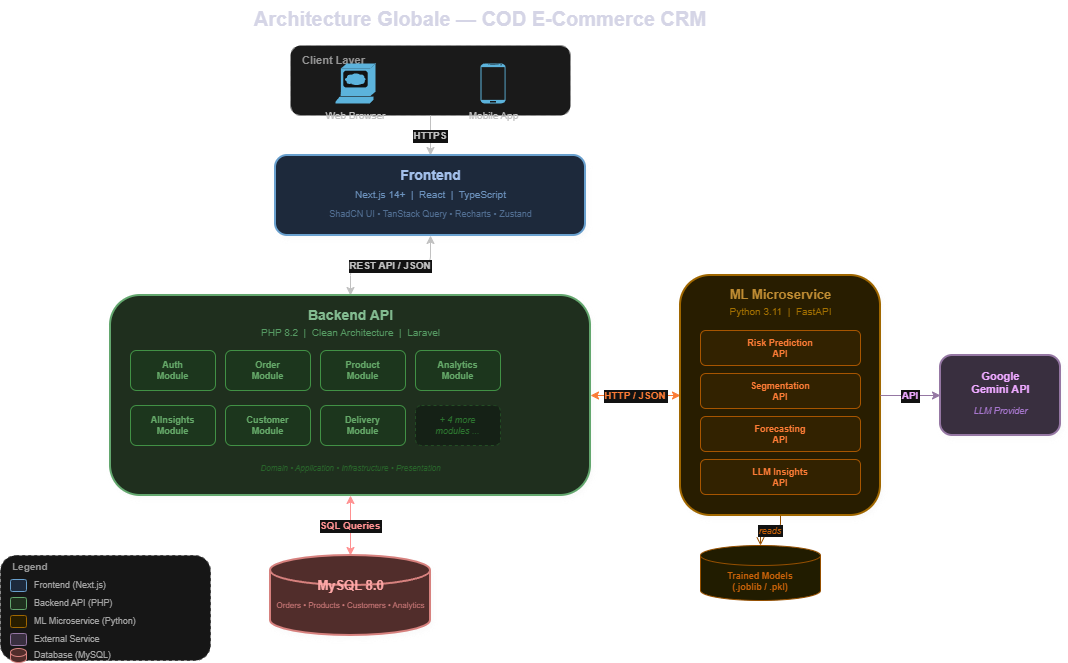
\includegraphics[width=\textwidth]{architecture_globale.drawio.png}
\caption{Architecture globale du syst\`{e}me}
\label{fig:architecture}
\end{figure}

Le syst\`{e}me repose sur une communication REST/JSON entre les composants. Le backend PHP (Clean Architecture, pattern Controller-Service-Repository) orchestre les \'{e}changes avec la base MySQL 8.0 (UTF8MB4 pour le multilingue arabe/fran\c{c}ais) et d\'{e}l\`{e}gue les traitements analytiques au microservice ML Python (FastAPI). Ce dernier int\`{e}gre \'{e}galement l'API Google Gemini (\texttt{gemini-2.0-flash}) pour la g\'{e}n\'{e}ration d'insights en langage naturel.

\section{Conception de la base de donn\'{e}es}

La base de donn\'{e}es MySQL comprend \textbf{12 tables} r\'{e}parties en 5 fichiers de migration, avec une architecture multi-tenant o\`{u} chaque table op\'{e}rationnelle est isol\'{e}e par \texttt{store\_id}.

\subsection{Sch\'{e}ma relationnel}

\begin{figure}[H]
\centering
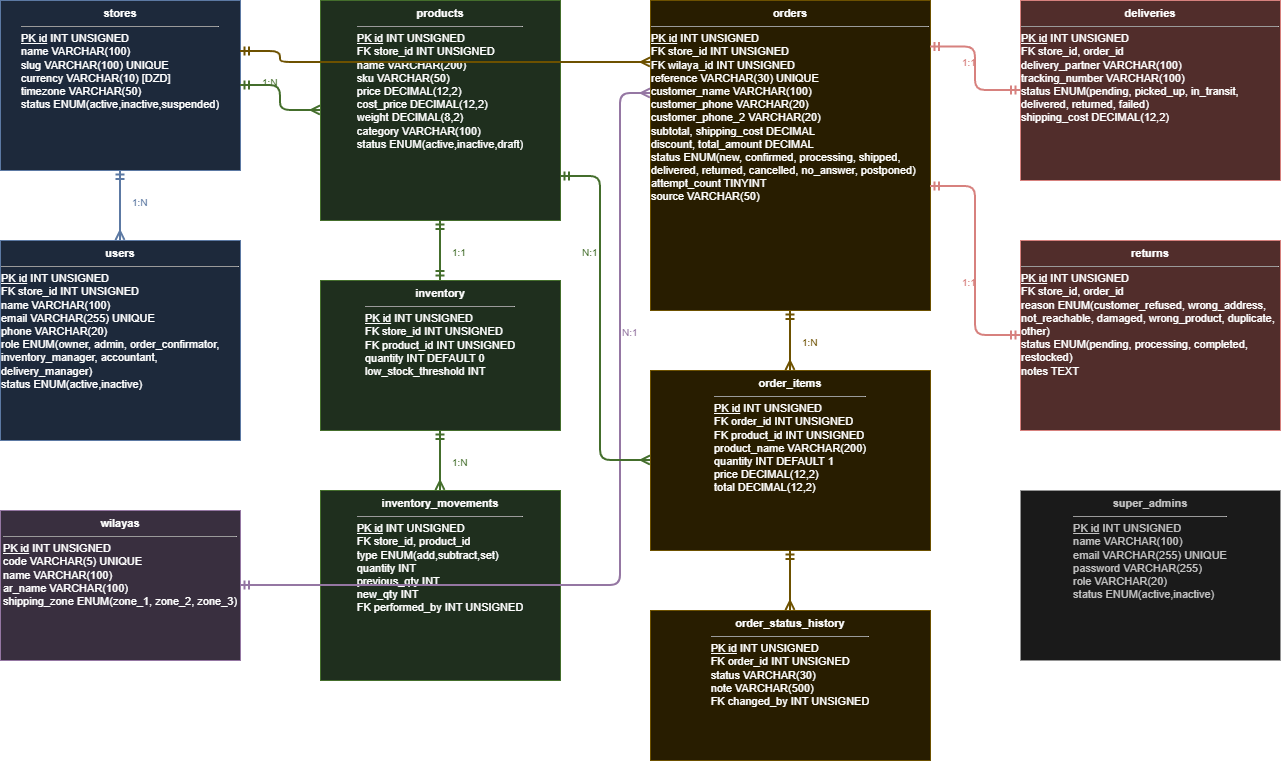
\includegraphics[width=\textwidth]{schema_base_donnees.drawio.png}
\caption{Sch\'{e}ma relationnel de la base de donn\'{e}es}
\label{fig:schema}
\end{figure}

\subsection{Tables principales}

\begin{table}[H]
\centering
\caption{Description des tables de la base de donn\'{e}es}
\label{tab:tables}
\begin{tabularx}{\textwidth}{l l X}
\toprule
\textbf{Table} & \textbf{Cl\'{e}s} & \textbf{Description} \\
\midrule
\texttt{stores} & PK: id & Magasins (racine multi-tenant) \\
\texttt{wilayas} & PK: id & 58 wilayas d'Alg\'{e}rie, 3 zones d'exp\'{e}dition \\
\texttt{users} & PK: id, FK: store\_id & Utilisateurs avec 6 r\^{o}les RBAC \\
\texttt{products} & PK: id, FK: store\_id & Catalogue produits (prix, cat\'{e}gorie, poids) \\
\texttt{inventory} & PK: id, FK: product\_id & Suivi des stocks avec seuil d'alerte \\
\texttt{inventory\_movements} & PK: id & Historique des mouvements de stock \\
\texttt{orders} & PK: id, FK: store\_id, wilaya\_id & Commandes avec 9 statuts possibles \\
\texttt{order\_items} & PK: id, FK: order\_id & Articles de commande \\
\texttt{order\_status\_history} & PK: id, FK: order\_id & Piste d'audit des changements de statut \\
\texttt{deliveries} & PK: id, FK: order\_id & Gestion des livraisons (6 statuts) \\
\texttt{returns} & PK: id, FK: order\_id & Gestion des retours (7 raisons) \\
\texttt{super\_admins} & PK: id & Administrateurs de la plateforme \\
\bottomrule
\end{tabularx}
\end{table}

\subsection{Cycle de vie d'une commande COD}

La table \texttt{orders} utilise un champ \texttt{status} de type ENUM avec 9 \'{e}tats possibles refl\'{e}tant le cycle de vie complet d'une commande COD :

\begin{figure}[H]
\centering
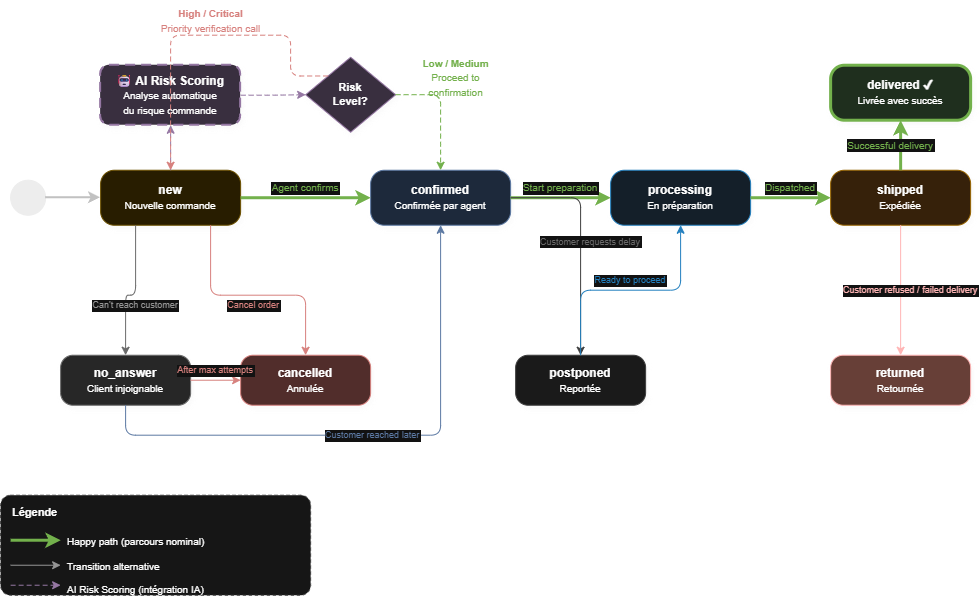
\includegraphics[width=\textwidth]{cycle_vie_commande.drawio.png}
\caption{Cycle de vie d'une commande COD avec int\'{e}gration IA}
\label{fig:order_states}
\end{figure}

\section{Architecture du module ML}

Le module ML est un microservice Python autonome communiquant avec le backend PHP via API REST.

\subsection{Int\'{e}gration IA dans le syst\`{e}me}

La figure \ref{fig:ai_integration} pr\'{e}sente les trois flux d'analyse IA int\'{e}gr\'{e}s dans le CRM, ainsi que le composant LLM pour la g\'{e}n\'{e}ration d'insights.

\begin{figure}[H]
\centering
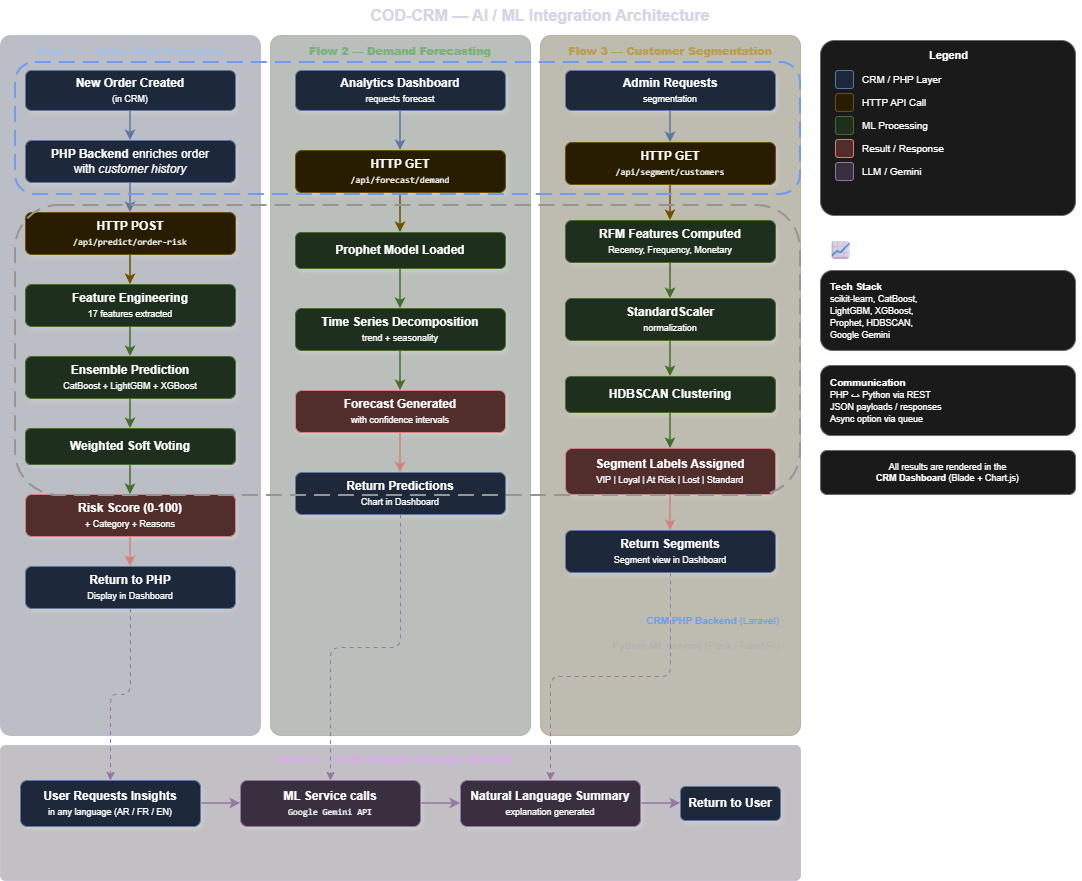
\includegraphics[width=\textwidth]{ai_integration.drawio.png}
\caption{Flux d'int\'{e}gration IA dans le CRM}
\label{fig:ai_integration}
\end{figure}

\subsection{Structure du microservice}

\begin{lstlisting}[language={}, caption={Arborescence du module ML}]
ml-service/
  app/
    main.py              # Point d'entree FastAPI
    config.py            # Configuration
    models/
      predictor.py       # Ensemble CatBoost+LightGBM+XGBoost
      segmenter.py       # Segmentation HDBSCAN
      forecaster.py      # Prevision Prophet
      features.py        # Ingenierie des features
    routes/
      predict.py         # Endpoints prediction
      segment.py         # Endpoints segmentation
      forecast.py        # Endpoints prevision
      insights.py        # Endpoints LLM
    services/
      ml_service.py      # Orchestrateur des modeles
      llm_service.py     # Integration Google Gemini
      data_service.py    # Chargement des donnees
  data/
    prepare_data.py      # Pipeline de preparation
    mapping.py           # Mapping Olist -> CRM
  train_all.py           # Script d'entrainement
  trained_models/        # Modeles sauvegardes
\end{lstlisting}

\subsection{Endpoints de l'API ML}

\begin{table}[H]
\centering
\caption{Endpoints REST du module ML}
\label{tab:endpoints}
\begin{tabularx}{\textwidth}{l l X}
\toprule
\textbf{M\'{e}thode} & \textbf{Endpoint} & \textbf{Description} \\
\midrule
POST & \texttt{/api/predict/order-risk} & Pr\'{e}diction du risque pour une commande \\
POST & \texttt{/api/predict/order-risk/batch} & Pr\'{e}diction en lot (batch) \\
GET & \texttt{/api/predict/model-info} & Information sur le mod\`{e}le \\
GET & \texttt{/api/segment/customers} & Segmentation des clients \\
GET & \texttt{/api/segment/summary} & R\'{e}sum\'{e} des segments \\
GET & \texttt{/api/forecast/demand} & Pr\'{e}vision de la demande \\
GET & \texttt{/api/forecast/categories} & Cat\'{e}gories disponibles \\
GET & \texttt{/api/insights/summary} & Insights g\'{e}n\'{e}r\'{e}s par LLM \\
GET & \texttt{/api/insights/recommendations} & Recommandations IA \\
\bottomrule
\end{tabularx}
\end{table}

\subsection{Int\'{e}gration avec le backend PHP}

Le backend PHP communique avec le module ML via un service d\'{e}di\'{e} (\texttt{AIInsightsService}) qui encapsule les appels HTTP :

\begin{lstlisting}[language=PHP, caption={Extrait du contr\^{o}leur PHP pour l'IA}]
// AIInsightsController.php
public function orderRisk(Request $request, int $id): Response
{
    // 1. Charger la commande depuis MySQL
    $order = $this->service->getOrderWithDetails($id);

    // 2. Enrichir avec l'historique client
    $enriched = $this->service->enrichWithHistory($order);

    // 3. Appeler le module ML Python
    $risk = $this->aiService->getOrderRisk($enriched);

    return Response::success($risk);
}
\end{lstlisting}


% ══════════════════════════════════════════════════════════════
% CHAPITRE 4 : REALISATION
% ══════════════════════════════════════════════════════════════
\chapter{R\'{e}alisation}

\section{Technologies utilis\'{e}es}

\begin{table}[H]
\centering
\caption{Stack technologique du projet}
\label{tab:stack}
\begin{tabularx}{\textwidth}{l l X}
\toprule
\textbf{Composant} & \textbf{Technologie} & \textbf{Version / D\'{e}tails} \\
\midrule
Frontend & Next.js (React) & 14+ avec TypeScript \\
Backend & PHP & 8.2+ (Clean Architecture) \\
Base de donn\'{e}es & MySQL & 8.0+ (UTF8MB4) \\
Module ML & Python / FastAPI & 3.11+ / FastAPI + Uvicorn \\
ML -- Classification & CatBoost & 1.2.7 \\
ML -- Classification & LightGBM & 4.5.0 \\
ML -- Classification & XGBoost & 2.1.3 \\
ML -- Clustering & HDBSCAN & 0.8.39 \\
ML -- S\'{e}ries temporelles & Prophet & (Meta) \\
ML -- Features & scikit-learn & 1.6.1 \\
LLM & Google Gemini API & gemini-2.0-flash \\
Conteneurisation & Docker & Python 3.11-slim \\
\bottomrule
\end{tabularx}
\end{table}

\section{Le CRM : Modules fonctionnels}

Le CRM est organis\'{e} en \textbf{11 modules} suivant le pattern Clean Architecture :

\begin{enumerate}
  \item \textbf{Auth} : Authentification JWT, gestion des sessions
  \item \textbf{User} : Gestion des utilisateurs avec 6 r\^{o}les (Owner, Admin, Confirmateur, Gestionnaire stock, Comptable, Gestionnaire livraisons)
  \item \textbf{Store} : Configuration multi-tenant
  \item \textbf{Product} : Catalogue produits avec SKU, cat\'{e}gories, prix
  \item \textbf{Inventory} : Gestion des stocks avec seuils d'alerte et historique des mouvements
  \item \textbf{Order} : Cycle de vie complet des commandes COD (9 statuts)
  \item \textbf{Delivery} : Suivi des livraisons avec partenaires et num\'{e}ros de tracking
  \item \textbf{Returns} : Gestion des retours avec 7 motifs de retour
  \item \textbf{Analytics} : Tableau de bord analytique (KPIs, tendances)
  \item \textbf{Storefront} : Vitrine en ligne publique
  \item \textbf{Admin} : Panel super-administrateur de la plateforme
\end{enumerate}

\section{Jeu de donn\'{e}es : Olist Brazilian E-Commerce}

En l'absence de donn\'{e}es r\'{e}elles de e-commerce alg\'{e}rien, nous avons utilis\'{e} le jeu de donn\'{e}es public \textbf{Olist Brazilian E-Commerce} \cite{olist2018} disponible sur Kaggle. Ce dataset contient :

\begin{itemize}
  \item \textbf{100 000+} commandes r\'{e}elles (2016--2018)
  \item Informations clients, produits, paiements, avis
  \item Donn\'{e}es g\'{e}ographiques (27 \'{e}tats br\'{e}siliens)
  \item Statuts de livraison (livr\'{e}, annul\'{e}, etc.)
\end{itemize}

\subsection{Transformation et mapping}

Un pipeline de transformation a \'{e}t\'{e} d\'{e}velopp\'{e} pour adapter les donn\'{e}es Olist au sch\'{e}ma CRM alg\'{e}rien :

\begin{table}[H]
\centering
\caption{Mapping des donn\'{e}es Olist vers le sch\'{e}ma CRM}
\label{tab:mapping}
\begin{tabularx}{\textwidth}{l l X}
\toprule
\textbf{Originale (Olist)} & \textbf{Transform\'{e}e (CRM)} & \textbf{Transformation} \\
\midrule
27 \'{e}tats br\'{e}siliens & 58 wilayas & Mapping \'{e}tat $\rightarrow$ wilaya \\
BRL (R\'{e}al) & DZD (Dinar) & Taux : 1 BRL = 27 DZD \\
\texttt{delivered} & \texttt{delivered} & \multirow{2}{*}{Mapping des statuts} \\
\texttt{canceled} & \texttt{cancelled} & \\
Cat\'{e}gories (PT) & Cat\'{e}gories (EN) & Traduction portugais $\rightarrow$ anglais \\
\bottomrule
\end{tabularx}
\end{table}

Apr\`{e}s transformation, le jeu de donn\'{e}es contient \textbf{99~441 commandes} avec un taux de livraison de \textbf{97,0\%}.

\section{R\'{e}entra\^{i}nement des mod\`{e}les}

Le syst\`{e}me est con\c{c}u pour permettre \`{a} l'entreprise d'importer ses propres donn\'{e}es et de r\'{e}entra\^{i}ner les mod\`{e}les. Les mod\`{e}les entra\^{i}n\'{e}s sur les donn\'{e}es Olist servent de d\'{e}faut, tandis que l'API de r\'{e}entra\^{i}nement permet une mise \`{a} jour sans intervention technique :

\begin{table}[H]
\centering
\caption{Endpoints de r\'{e}entra\^{i}nement et gestion des mod\`{e}les}
\label{tab:retrain_endpoints}
\begin{tabularx}{\textwidth}{l l X}
\toprule
\textbf{M\'{e}thode} & \textbf{Endpoint} & \textbf{Description} \\
\midrule
POST & \texttt{/api/retrain/upload-and-train} & Importer un CSV et r\'{e}entra\^{i}ner tous les mod\`{e}les \\
POST & \texttt{/api/retrain/restore-defaults} & Restaurer les mod\`{e}les par d\'{e}faut (sauvegard\'{e}s) \\
GET & \texttt{/api/retrain/metrics} & Consulter les m\'{e}triques d'\'{e}valuation \\
GET & \texttt{/api/retrain/data-format} & Obtenir le format CSV attendu \\
\bottomrule
\end{tabularx}
\end{table}

Le processus de r\'{e}entra\^{i}nement :
\begin{enumerate}
  \item Sauvegarde automatique des mod\`{e}les actuels dans un r\'{e}pertoire de backup
  \item Validation et transformation du CSV import\'{e} (adaptation automatique des noms de colonnes)
  \item Entra\^{i}nement des trois mod\`{e}les (risque, segmentation, pr\'{e}vision)
  \item Sauvegarde des m\'{e}triques d'\'{e}valuation en JSON
  \item Rechargement automatique des mod\`{e}les dans le service en cours d'ex\'{e}cution
  \item Possibilit\'{e} de restaurer les mod\`{e}les pr\'{e}c\'{e}dents en cas de r\'{e}gression
\end{enumerate}

Les m\'{e}triques d'\'{e}valuation (AUC-ROC, F1-Score, MAE, RMSE, matrice de confusion) sont persist\'{e}es dans un fichier \texttt{metrics.json} apr\`{e}s chaque entra\^{i}nement, permettant un suivi historique des performances.


% ══════════════════════════════════════════════════════════════
% CHAPITRE 5 : MODELES ML, EVALUATION ET RESULTATS
% ══════════════════════════════════════════════════════════════
\chapter{Mod\`{e}les de Machine Learning, \'{E}valuation et R\'{e}sultats}

Ce chapitre pr\'{e}sente les trois mod\`{e}les de ML d\'{e}velopp\'{e}s, leur comparaison rigoureuse et l'interpr\'{e}tation des r\'{e}sultats dans une perspective d'aide \`{a} la d\'{e}cision.

\section{Pipeline Machine Learning}

La figure \ref{fig:ml_pipeline} illustre le pipeline complet, de la pr\'{e}paration des donn\'{e}es au d\'{e}ploiement des mod\`{e}les.

\begin{figure}[H]
\centering
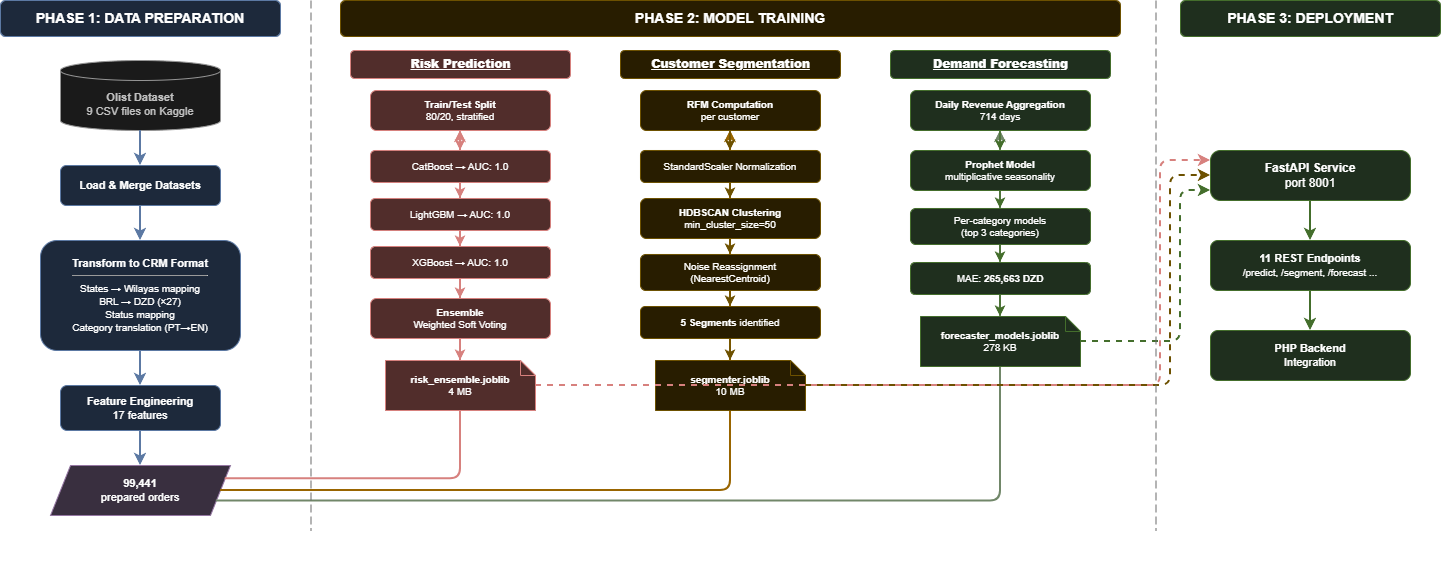
\includegraphics[width=\textwidth]{ml_pipeline.drawio.png}
\caption{Pipeline Machine Learning : de la donn\'{e}e brute au d\'{e}ploiement}
\label{fig:ml_pipeline}
\end{figure}

\section{Pr\'{e}diction du risque de livraison}

\subsection{Formulation du probl\`{e}me}

Le probl\`{e}me est formul\'{e} comme une \textbf{classification binaire} : pr\'{e}dire si une commande sera livr\'{e}e avec succ\`{e}s ($y=1$) ou \'{e}chouera ($y=0$).

\subsection{Ing\'{e}nierie des features}

\`{A} partir des donn\'{e}es brutes de commande, \textbf{17 features} sont extraites, regroup\'{e}es en 5 cat\'{e}gories :

\begin{table}[H]
\centering
\caption{Features utilis\'{e}es pour la pr\'{e}diction du risque}
\label{tab:features}
\begin{tabularx}{\textwidth}{l l X}
\toprule
\textbf{Cat\'{e}gorie} & \textbf{Feature} & \textbf{Description} \\
\midrule
\multirow{4}{*}{Temporelles} & hour\_of\_day & Heure de la commande (0--23) \\
 & day\_of\_week & Jour de la semaine (0--6) \\
 & month & Mois (1--12) \\
 & is\_weekend & Commande le week-end (0/1) \\
\midrule
\multirow{4}{*}{Valeur} & order\_value & Montant total (DZD) \\
 & shipping\_cost & Frais de livraison \\
 & discount & Remise appliqu\'{e}e \\
 & subtotal & Sous-total \\
\midrule
\multirow{1}{*}{Produit} & n\_items & Nombre d'articles \\
\midrule
\multirow{4}{*}{Client} & has\_alt\_phone & T\'{e}l\'{e}phone alternatif (0/1) \\
 & is\_repeat\_customer & Client r\'{e}current (0/1) \\
 & customer\_order\_count & Historique commandes \\
 & customer\_success\_rate & Taux de succ\`{e}s historique \\
\midrule
\multirow{4}{*}{Contextuelles} & region\_success\_rate & Taux de succ\`{e}s r\'{e}gional \\
 & category\_success\_rate & Taux de succ\`{e}s cat\'{e}gorie \\
 & estimated\_delivery\_days & D\'{e}lai estim\'{e} (jours) \\
 & avg\_product\_weight & Poids moyen du colis \\
\bottomrule
\end{tabularx}
\end{table}

\subsection{Mod\`{e}les entra\^{i}n\'{e}s et comparaison}

Trois mod\`{e}les de gradient boosting ont \'{e}t\'{e} entra\^{i}n\'{e}s individuellement puis combin\'{e}s en un ensemble par vote pond\'{e}r\'{e}. La r\'{e}partition des donn\'{e}es est de 80\% entra\^{i}nement / 20\% test, avec stratification.

\begin{table}[H]
\centering
\caption{R\'{e}partition des donn\'{e}es d'entra\^{i}nement et de test}
\label{tab:split}
\begin{tabularx}{\textwidth}{l r r r}
\toprule
\textbf{Ensemble} & \textbf{Total} & \textbf{Livr\'{e}es ($y=1$)} & \textbf{\'{E}chou\'{e}es ($y=0$)} \\
\midrule
Entra\^{i}nement (80\%) & 79~552 & 77~182 (97,0\%) & 2~370 (3,0\%) \\
Test (20\%) & 19~889 & 19~296 (97,0\%) & 593 (3,0\%) \\
\midrule
\textbf{Total} & \textbf{99~441} & \textbf{96~478} & \textbf{2~963} \\
\bottomrule
\end{tabularx}
\end{table}

\subsubsection{R\'{e}sultats comparatifs}

\begin{table}[H]
\centering
\caption{Comparaison des performances des mod\`{e}les de classification}
\label{tab:comparison}
\begin{tabularx}{\textwidth}{l *{5}{>{\centering\arraybackslash}X}}
\toprule
\textbf{Mod\`{e}le} & \textbf{AUC-ROC} & \textbf{Accuracy} & \textbf{Pr\'{e}cision} & \textbf{Rappel} & \textbf{F1-Score} \\
\midrule
CatBoost & 1.0000 & 0.9982 & 0.9999 & 0.9983 & 0.9991 \\
LightGBM & 1.0000 & 0.9983 & 0.9992 & 0.9990 & 0.9991 \\
XGBoost & 1.0000 & 0.9983 & 0.9999 & 0.9983 & 0.9991 \\
\midrule
\textbf{Ensemble} & \textbf{1.0000} & \textbf{0.9983} & \textbf{0.9998} & \textbf{0.9984} & \textbf{0.9991} \\
\bottomrule
\end{tabularx}
\end{table}

\subsubsection{Matrice de confusion (Ensemble)}

\begin{table}[H]
\centering
\caption{Matrice de confusion du mod\`{e}le ensemble sur l'ensemble de test}
\label{tab:confusion}
\begin{tabular}{l|c|c|}
\cline{2-3}
 & \textbf{Pr\'{e}dit : \'{E}chou\'{e}e} & \textbf{Pr\'{e}dit : Livr\'{e}e} \\
\hline
\multicolumn{1}{|l|}{\textbf{R\'{e}el : \'{E}chou\'{e}e}} & 590 (VN) & 3 (FP) \\
\hline
\multicolumn{1}{|l|}{\textbf{R\'{e}el : Livr\'{e}e}} & 31 (FN) & 19~265 (VP) \\
\hline
\end{tabular}
\end{table}

\subsubsection{Analyse des r\'{e}sultats}

Les trois mod\`{e}les atteignent des performances tr\`{e}s \'{e}lev\'{e}es (AUC-ROC = 1.0), ce qui s'explique par :

\begin{enumerate}
  \item \textbf{Le d\'{e}s\'{e}quilibre des classes} : Avec 97\% de commandes livr\'{e}es, les features capturent efficacement les 3\% d'\'{e}checs qui pr\'{e}sentent des caract\'{e}ristiques distinctives.
  \item \textbf{La richesse des features contextuelles} : Les taux de succ\`{e}s r\'{e}gionaux et par cat\'{e}gorie, calcul\'{e}s \`{a} partir des donn\'{e}es historiques, sont fortement corr\'{e}l\'{e}s au r\'{e}sultat.
  \item \textbf{La qualit\'{e} du jeu de donn\'{e}es Olist} : Les donn\'{e}es sont compl\`{e}tes avec peu de valeurs manquantes.
\end{enumerate}

\textbf{Note importante} : Ces performances sont mesur\'{e}es sur les donn\'{e}es Olist transform\'{e}es. En production avec des donn\'{e}es r\'{e}elles alg\'{e}riennes, les performances pourraient varier. Un r\'{e}entra\^{i}nement sur les donn\'{e}es r\'{e}elles sera n\'{e}cessaire.

L'ensemble par vote pond\'{e}r\'{e} est retenu car il offre une robustesse accrue : si un mod\`{e}le individuel se trompe, les deux autres peuvent compenser.

\subsection{Cat\'{e}gories de risque et aide \`{a} la d\'{e}cision}

Le score de risque (0--100) est traduit en cat\'{e}gories actionnables :

\begin{table}[H]
\centering
\caption{Cat\'{e}gories de risque et recommandations}
\label{tab:risk_categories}
\begin{tabularx}{\textwidth}{l l X}
\toprule
\textbf{Score} & \textbf{Cat\'{e}gorie} & \textbf{Action recommand\'{e}e} \\
\midrule
0--25 & Critique & V\'{e}rifier le client par t\'{e}l\'{e}phone. Confirmer l'adresse. \\
25--50 & \'{E}lev\'{e} & Appel de confirmation prioritaire. \\
50--75 & Moyen & Traitement standard, surveillance accrue. \\
75--100 & Faible & Proc\'{e}der normalement. \\
\bottomrule
\end{tabularx}
\end{table}


\section{Segmentation client par HDBSCAN}

\subsection{M\'{e}thodologie}

La segmentation utilise l'analyse RFM (Recency, Frequency, Monetary) comme features d'entr\'{e}e pour l'algorithme HDBSCAN :

\begin{enumerate}
  \item Calcul des m\'{e}triques RFM pour chaque client
  \item Normalisation par \texttt{StandardScaler}
  \item Clustering HDBSCAN avec \texttt{min\_cluster\_size=50}
  \item R\'{e}assignation des points de bruit via \texttt{NearestCentroid}
  \item \'{E}tiquetage des clusters selon les statistiques RFM
\end{enumerate}

\subsection{R\'{e}sultats de la segmentation}

HDBSCAN a identifi\'{e} automatiquement \textbf{5 clusters} parmi \textbf{96~096 clients} :

\begin{table}[H]
\centering
\caption{Segments clients identifi\'{e}s par HDBSCAN}
\label{tab:segments}
\begin{tabularx}{\textwidth}{l r r X}
\toprule
\textbf{Segment} & \textbf{Clients} & \textbf{\%} & \textbf{Description} \\
\midrule
VIP & 3~673 & 3,8\% & Clients \`{a} haute valeur, achats fr\'{e}quents et r\'{e}cents \\
Loyal & 252 & 0,3\% & Clients r\'{e}guliers avec bon historique d'achat \\
\`{A} risque & 2~736 & 2,8\% & Clients pr\'{e}c\'{e}demment actifs montrant un d\'{e}clin \\
Perdu & 441 & 0,5\% & Clients inactifs sans achats r\'{e}cents \\
Standard & 88~994 & 92,6\% & Clients occasionnels (majorit\'{e}) \\
\bottomrule
\end{tabularx}
\end{table}

\subsection{Interpr\'{e}tation pour l'aide \`{a} la d\'{e}cision}

La segmentation permet des actions cibl\'{e}es :

\begin{itemize}
  \item \textbf{VIP (3,8\%)} : Programme de fid\'{e}lit\'{e}, offres exclusives, service client prioritaire
  \item \textbf{Loyal (0,3\%)} : Maintien de la relation, cross-selling
  \item \textbf{\`{A} risque (2,8\%)} : Campagnes de r\'{e}activation, offres promotionnelles
  \item \textbf{Perdu (0,5\%)} : Analyse des causes d'abandon
  \item \textbf{Standard (92,6\%)} : Strat\'{e}gies de conversion en clients r\'{e}currents
\end{itemize}

\textbf{Limite du dataset} : Le dataset Olist contient majoritairement des clients \`{a} achat unique (fr\'{e}quence = 1), ce qui r\'{e}duit la variabilit\'{e} de la segmentation. Avec des donn\'{e}es r\'{e}elles de COD alg\'{e}rien (o\`{u} les clients r\'{e}currents sont plus fr\'{e}quents), la segmentation serait plus diff\'{e}renci\'{e}e.


\section{Pr\'{e}vision de la demande avec Prophet}

\subsection{Pr\'{e}paration des donn\'{e}es temporelles}

Les commandes livr\'{e}es sont agr\'{e}g\'{e}es par jour pour cr\'{e}er une s\'{e}rie temporelle du chiffre d'affaires quotidien sur \textbf{714 jours}.

\begin{itemize}
  \item S\'{e}rie : Chiffre d'affaires quotidien en DZD
  \item P\'{e}riode : 714 jours
  \item Entra\^{i}nement : 654 jours (premiers 91,6\%)
  \item Test : 60 derniers jours (8,4\%)
\end{itemize}

\subsection{Configuration du mod\`{e}le Prophet}

\begin{lstlisting}[language=Python, caption={Configuration du mod\`{e}le Prophet}]
model = Prophet(
    yearly_seasonality=True,
    weekly_seasonality=True,
    daily_seasonality=False,
    changepoint_prior_scale=0.05,
    seasonality_prior_scale=10.0,
    seasonality_mode="multiplicative",
)
\end{lstlisting}

Le mode multiplicatif est choisi car l'amplitude des variations saisonni\`{e}res cro\^{i}t proportionnellement au niveau de la s\'{e}rie.

\subsection{Comparaison Prophet vs. Moyenne Mobile}

Pour \'{e}valuer la valeur ajout\'{e}e de Prophet, nous le comparons \`{a} une baseline na\"{i}ve (moyenne mobile 7 jours) :

\begin{table}[H]
\centering
\caption{Comparaison Prophet vs. Moyenne Mobile (pr\'{e}vision \`{a} 60 jours)}
\label{tab:forecast_comparison}
\begin{tabularx}{\textwidth}{l *{3}{>{\centering\arraybackslash}X}}
\toprule
\textbf{Mod\`{e}le} & \textbf{MAE (DZD)} & \textbf{RMSE (DZD)} & \textbf{Am\'{e}lioration} \\
\midrule
Moyenne Mobile (7j) & 301~401 & 371~511 & --- (baseline) \\
\textbf{Prophet} & \textbf{265~663} & \textbf{363~848} & \textbf{11,9\%} (MAE) \\
\bottomrule
\end{tabularx}
\end{table}

Prophet surpasse la baseline avec une r\'{e}duction de \textbf{11,9\%} du MAE et de \textbf{2,1\%} du RMSE. Le mod\`{e}le capture les motifs saisonniers hebdomadaires et les tendances que la moyenne mobile ne peut pas mod\'{e}liser.

\subsection{Mod\`{e}les par cat\'{e}gorie}

En plus du mod\`{e}le global, des mod\`{e}les Prophet sp\'{e}cifiques ont \'{e}t\'{e} entra\^{i}n\'{e}s pour les 3 cat\'{e}gories principales :

\begin{table}[H]
\centering
\caption{Mod\`{e}les de pr\'{e}vision par cat\'{e}gorie de produit}
\label{tab:forecast_cats}
\begin{tabularx}{\textwidth}{l X}
\toprule
\textbf{Cat\'{e}gorie} & \textbf{Description} \\
\midrule
all (global) & Pr\'{e}vision du chiffre d'affaires total quotidien \\
bed\_bath\_table & Linge de maison, salle de bain, d\'{e}coration \\
health\_beauty & Sant\'{e} et beaut\'{e} \\
sports\_leisure & Sports et loisirs \\
\bottomrule
\end{tabularx}
\end{table}


\section{Int\'{e}gration LLM : Google Gemini}

Le module d'insights utilise l'API Google Gemini (\texttt{gemini-2.0-flash}) pour g\'{e}n\'{e}rer des explications et recommandations en langage naturel dans trois langues :

\begin{itemize}
  \item \textbf{Arabe} : Langue officielle
  \item \textbf{Fran\c{c}ais} : Langue d'affaires
  \item \textbf{Anglais} : Langue technique
\end{itemize}

Les endpoints LLM fournissent :
\begin{enumerate}
  \item \textbf{R\'{e}sum\'{e}s de p\'{e}riode} : Synth\`{e}se des KPIs avec analyse des tendances
  \item \textbf{Explication du risque} : Explication en langage naturel du score de risque d'une commande
  \item \textbf{Recommandations} : Suggestions d'actions commerciales contextualis\'{e}es
\end{enumerate}

\section{Synth\`{e}se comparative des mod\`{e}les}

\begin{table}[H]
\centering
\caption{Synth\`{e}se des mod\`{e}les d\'{e}velopp\'{e}s}
\label{tab:synthesis}
\begin{tabularx}{\textwidth}{l l l X}
\toprule
\textbf{T\^{a}che} & \textbf{Type} & \textbf{Mod\`{e}le(s)} & \textbf{M\'{e}trique cl\'{e}} \\
\midrule
Risque livraison & Classification & CatBoost + LightGBM + XGBoost & AUC-ROC = 1.0, F1 = 0.999 \\
Segmentation & Clustering & HDBSCAN + RFM & 5 clusters, silhouette auto \\
Pr\'{e}vision demande & S\'{e}rie temporelle & Prophet & MAE = 265~663 DZD \\
Insights NL & G\'{e}n\'{e}ratif & Google Gemini & Multilingue (AR/FR/EN) \\
\bottomrule
\end{tabularx}
\end{table}


% ══════════════════════════════════════════════════════════════
% CONCLUSION GENERALE
% ══════════════════════════════════════════════════════════════
\chapter*{Conclusion G\'{e}n\'{e}rale}
\addcontentsline{toc}{chapter}{Conclusion G\'{e}n\'{e}rale}

Ce projet a permis de concevoir et de d\'{e}velopper un CRM intelligent pour le e-commerce COD en Alg\'{e}rie, int\'{e}grant un module de pr\'{e}diction des ventes bas\'{e} sur le Machine Learning.

\textbf{Les contributions principales sont :}

\begin{enumerate}
  \item \textbf{Un CRM complet} : 12 tables, 11 modules fonctionnels, architecture multi-tenant avec gestion fine des r\^{o}les (RBAC \`{a} 6 r\^{o}les).

  \item \textbf{Une base de donn\'{e}es rigoureusement con\c{c}ue} : Sch\'{e}ma normalis\'{e} avec int\'{e}grit\'{e} r\'{e}f\'{e}rentielle, pistes d'audit, support multilingue (UTF8MB4), et isolation multi-tenant par \texttt{store\_id}.

  \item \textbf{Un module ML multi-t\^{a}ches} :
  \begin{itemize}
    \item Pr\'{e}diction du risque par un ensemble de 3 mod\`{e}les (CatBoost, LightGBM, XGBoost) atteignant un F1-Score de 0.999
    \item Segmentation automatique des clients par HDBSCAN identifiant 5 profils distincts
    \item Pr\'{e}vision de la demande par Prophet avec une am\'{e}lioration de 11,9\% du MAE par rapport \`{a} une baseline nave
  \end{itemize}

  \item \textbf{Une comparaison rigoureuse} : Trois algorithmes de gradient boosting compar\'{e}s sur 5 m\'{e}triques (AUC-ROC, Accuracy, Pr\'{e}cision, Rappel, F1-Score), et Prophet compar\'{e} \`{a} une moyenne mobile sur MAE et RMSE.

  \item \textbf{Une architecture modulaire} : Le microservice ML (FastAPI) communique avec le backend PHP via API REST, permettant un d\'{e}ploiement ind\'{e}pendant et un passage \`{a} l'\'{e}chelle.
\end{enumerate}

\textbf{Perspectives :}

\begin{itemize}
  \item \textbf{Donn\'{e}es r\'{e}elles} : R\'{e}entra\^{i}ner les mod\`{e}les sur les donn\'{e}es r\'{e}elles du e-commerce alg\'{e}rien pour des performances repr\'{e}sentatives.
  \item \textbf{Mod\`{e}les deep learning} : Explorer les architectures Transformer (TabTransformer) pour les donn\'{e}es tabulaires et les mod\`{e}les N-BEATS/TFT pour la pr\'{e}vision temporelle.
  \item \textbf{Apprentissage en ligne} : Mettre \`{a} jour les mod\`{e}les en continu avec les nouvelles commandes.
  \item \textbf{A/B testing} : Mesurer l'impact r\'{e}el des recommandations ML sur le taux de livraison.
\end{itemize}


% ══════════════════════════════════════════════════════════════
% BIBLIOGRAPHIE
% ══════════════════════════════════════════════════════════════
\begin{thebibliography}{99}
\addcontentsline{toc}{chapter}{Bibliographie}

\bibitem{chen2016xgboost}
T. Chen and C. Guestrin, ``XGBoost: A Scalable Tree Boosting System,'' in \textit{Proceedings of the 22nd ACM SIGKDD International Conference on Knowledge Discovery and Data Mining}, pp. 785--794, 2016.

\bibitem{ke2017lightgbm}
G. Ke, Q. Meng, T. Finley, T. Wang, W. Chen, W. Ma, Q. Ye, and T.-Y. Liu, ``LightGBM: A Highly Efficient Gradient Boosting Decision Tree,'' in \textit{Advances in Neural Information Processing Systems 30}, pp. 3146--3154, 2017.

\bibitem{prokhorenkova2018catboost}
L. Prokhorenkova, G. Gusev, A. Vorobev, A. V. Dorogush, and A. Gulin, ``CatBoost: Unbiased Boosting with Categorical Features,'' in \textit{Advances in Neural Information Processing Systems 31}, pp. 6638--6648, 2018.

\bibitem{taylor2018forecasting}
S. J. Taylor and B. Letham, ``Forecasting at Scale,'' \textit{The American Statistician}, vol. 72, no. 1, pp. 37--45, 2018.

\bibitem{mcinnes2017hdbscan}
L. McInnes, J. Healy, and S. Astels, ``hdbscan: Hierarchical density based clustering,'' \textit{Journal of Open Source Software}, vol. 2, no. 11, p. 205, 2017.

\bibitem{grinsztajn2022tree}
L. Grinsztajn, E. Oyallon, and G. Varoquaux, ``Why do tree-based models still outperform deep learning on tabular data?'' in \textit{Advances in Neural Information Processing Systems 35}, 2022.

\bibitem{olist2018}
Olist, ``Brazilian E-Commerce Public Dataset by Olist,'' Kaggle, 2018. [Online]. Available: \url{https://www.kaggle.com/datasets/olistbr/brazilian-ecommerce}

\end{thebibliography}


% ══════════════════════════════════════════════════════════════
% ANNEXES
% ══════════════════════════════════════════════════════════════
\appendix
\chapter{Annexe : Exemple de requ\^{e}te et r\'{e}ponse de l'API}

\section{Pr\'{e}diction du risque d'une commande}

\begin{lstlisting}[language={}, caption={Requ\^{e}te POST /api/predict/order-risk}]
{
  "customer_name": "Ahmed Benali",
  "total_amount": 3000,
  "customer_order_count": 5,
  "customer_success_rate": 1.0,
  "is_repeat_customer": true,
  "customer_phone_2": "0666111222"
}
\end{lstlisting}

\begin{lstlisting}[language={}, caption={R\'{e}ponse de l'API de pr\'{e}diction}]
{
  "success": true,
  "data": {
    "score": 67.9,
    "category": "medium",
    "success_probability": 0.6794,
    "reasons": [
      "Region has low historical delivery success rate",
      "Product category has high return rate"
    ],
    "recommendation": "Standard processing.
      Monitor delivery status closely.",
    "model_scores": {
      "catboost": 92.1,
      "lightgbm": 12.7,
      "xgboost": 99.0
    }
  }
}
\end{lstlisting}

\section{Pr\'{e}vision de la demande}

\begin{lstlisting}[language={}, caption={R\'{e}ponse GET /api/forecast/demand?category=all\&periods=7}]
{
  "success": true,
  "data": {
    "category": "all",
    "periods": 7,
    "predictions": [
      {"ds": "2018-08-30", "yhat": 728927.35,
       "yhat_lower": 479230.78, "yhat_upper": 981872.42},
      {"ds": "2018-08-31", "yhat": 704937.78,
       "yhat_lower": 435953.28, "yhat_upper": 960256.39},
      {"ds": "2018-09-01", "yhat": 470569.50,
       "yhat_lower": 207655.72, "yhat_upper": 722730.63}
    ]
  }
}
\end{lstlisting}

\end{document}
